\section{Interface Design}
\subsection{User Flow and Mockups}

The LiftDrop application features distinct interfaces for different stages of the delivery process. Below are the key mockups organized by functionality.

\subsubsection{Authentication Flow}

The authentication flow allows users to securely access the LiftDrop system.

\begin{figure}[H]
    \centering
    \begin{subfigure}[b]{0.44\textwidth}
        \centering
        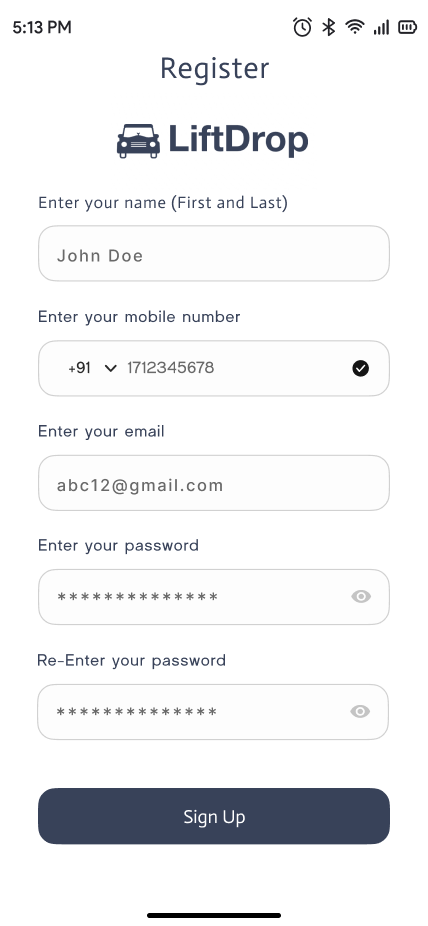
\includegraphics[width=\textwidth]{images/registration.png}
        \caption{User registration screen}
        \label{fig:registration}
    \end{subfigure}
    \hfill
    \begin{subfigure}[b]{0.44\textwidth}
        \centering
        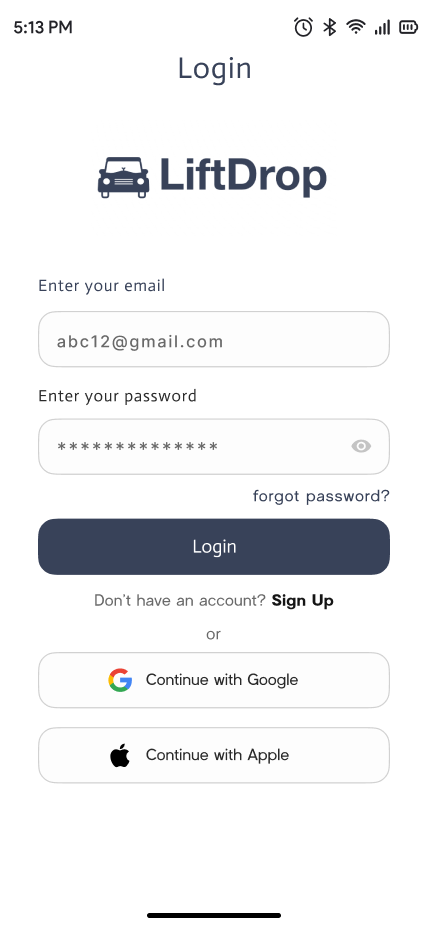
\includegraphics[width=\textwidth]{images/login.png}
        \caption{User login screen}
        \label{fig:login}
    \end{subfigure}
    \caption{Authentication flow screens for LiftDrop}
    \label{fig:auth_flow}
\end{figure}

\textbf{Registration Screen (\ref{fig:registration}):}  
Allows new users to create an account by entering essential information such as name, email, and password. This screen initiates access to the LiftDrop platform.

\textbf{Login Screen (\ref{fig:login}):}  
Enables users to securely log in using their credentials. The layout emphasizes simplicity and quick access.


\subsubsection{Courier Flow}

These screens illustrate the courier's working states, from availability to delivery.

\begin{figure}[H]
    \centering
    \begin{subfigure}[b]{0.48\textwidth}
        \centering
        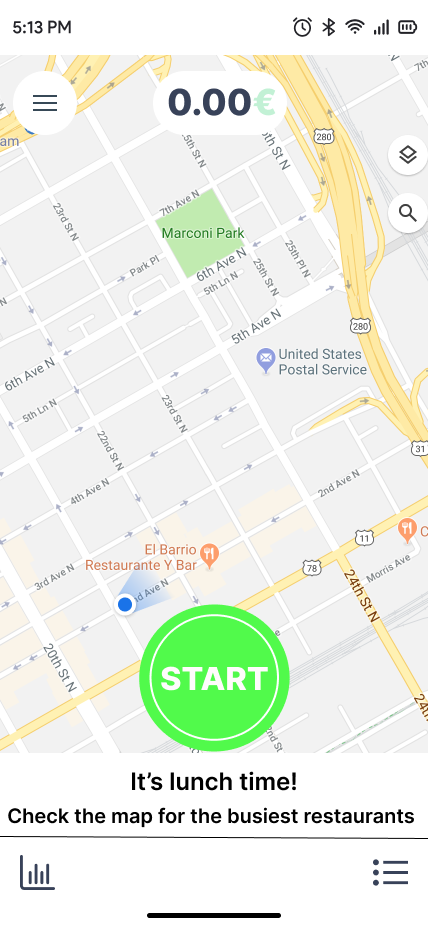
\includegraphics[width=\textwidth]{images/go_screen.png}
        \caption{Active status screen while courier is idle}
        \label{fig:go_screen}
    \end{subfigure}
    \hfill
    \begin{subfigure}[b]{0.48\textwidth}
        \centering
        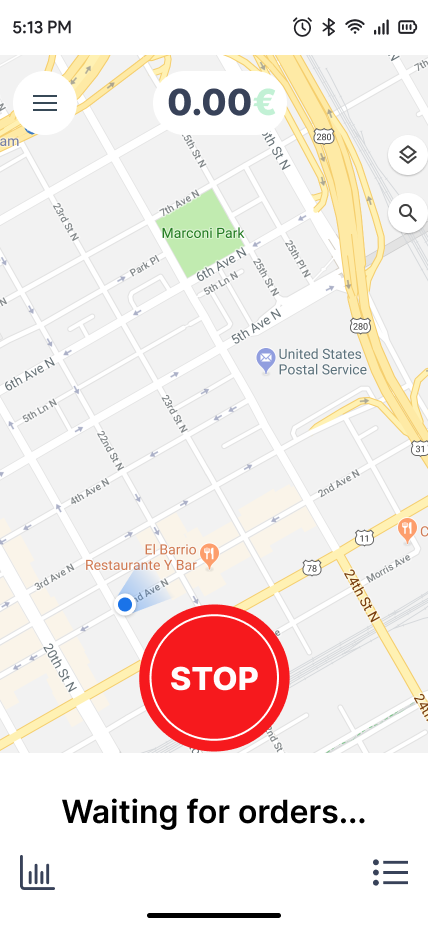
\includegraphics[width=\textwidth]{images/waiting_screen.png}
        \caption{Waiting screen during order availability check}
        \label{fig:waiting_screen}
    \end{subfigure}
    \caption{Courier status screens showing different working states}
    \label{fig:courier_status1}
\end{figure}

\textbf{Go Screen (\ref{fig:go_screen}):}  
Screen before the courier starts waiting for orders. A central status toggle makes it easy to go online or offline.

\textbf{Waiting Screen (\ref{fig:waiting_screen}):}  
Displays a waiting state while the system checks for nearby delivery requests. It reassures the user that the system is searching in the background.

\begin{figure}[H]
    \centering
    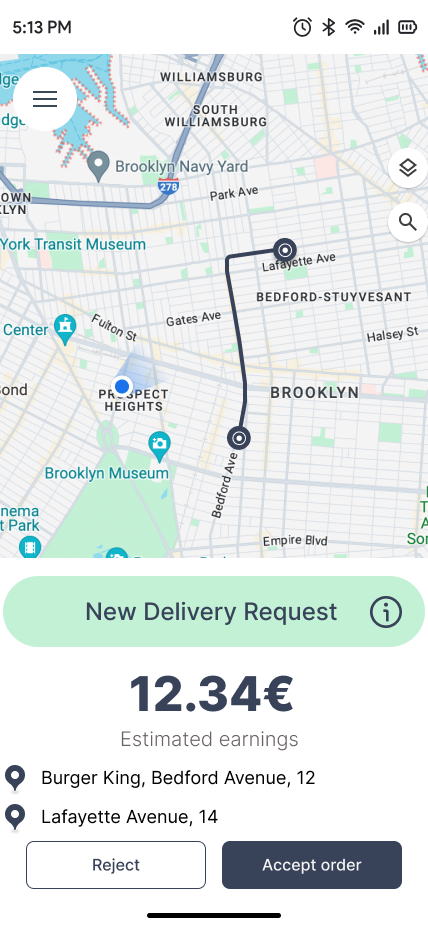
\includegraphics[width=0.6\textwidth]{images/delivery_request.png}
    \caption{New delivery request notification with order details and action buttons}
    \label{fig:delivery_request}
\end{figure}

\textbf{Delivery Request Notification (\ref{fig:delivery_request}):}  
Shows an incoming delivery request with pickup and drop-off addresses, estimated distance, and action buttons to accept or decline. It’s designed for quick decision-making and clarity.

\begin{figure}[H]
    \centering
    \begin{subfigure}[b]{0.48\textwidth}
        \centering
        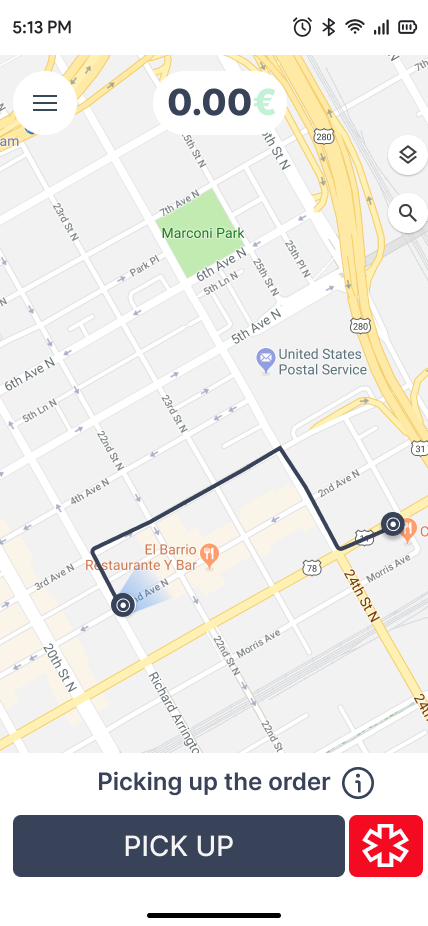
\includegraphics[width=\textwidth]{images/pickup_order_screen.png}
        \caption{Pickup Confirmation Screen}
        \label{fig:pickup_order}
    \end{subfigure}
    \hfill
    \begin{subfigure}[b]{0.48\textwidth}
        \centering
        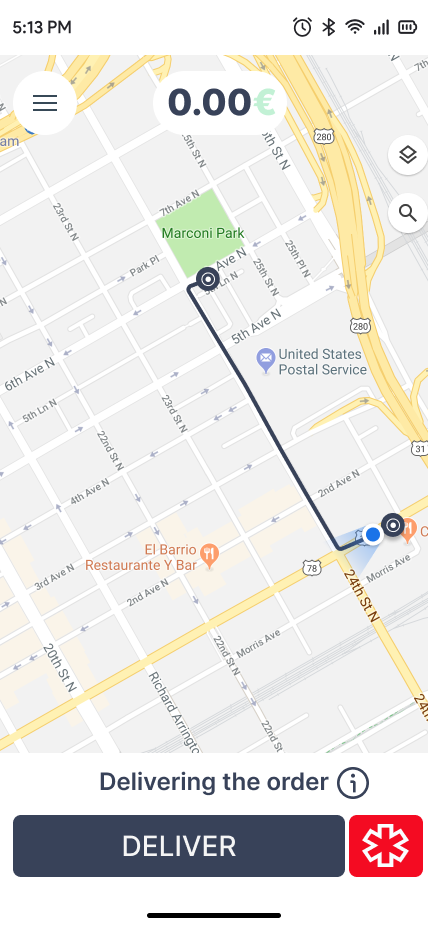
\includegraphics[width=\textwidth]{images/deliver_order_screen.png}
        \caption{Delivery Confirmation Screen}
        \label{fig:deliver_order}
    \end{subfigure}
    \caption{Courier delivery journey screens during different phases of the delivery}
    \label{fig:courier_journey}
\end{figure}

\textbf{Pickup Screen (\ref{fig:pickup_order}):}  
Provides order pickup instructions and customer location. It includes a confirmation action once the parcel is collected.

\textbf{Delivery Screen (\ref{fig:deliver_order}):}  
Guides the courier to the drop-off location. Includes proof-of-delivery options like signature or photo, depending on the order.
